\documentclass{standalone}
%----------------------------------------------------------------------%
%%% TikZ %%%
\usepackage{tikz}
\usetikzlibrary{calc}
\usetikzlibrary{intersections}
%----------------------------------------------------------------------%

\begin{document}

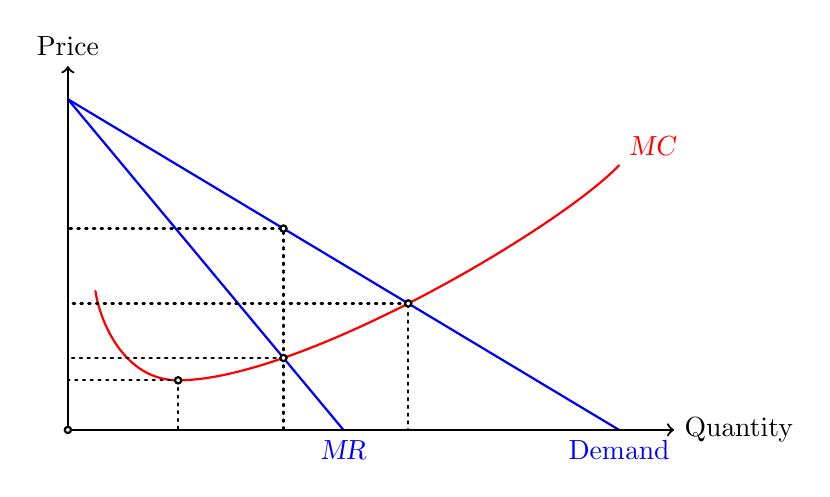
\begin{tikzpicture}[scale=0.7,yscale=0.6,thick,line cap=round]
	\tikzstyle{bai}=[solid,circle,draw=black,inner sep=.8pt,fill=white];
	%% Demand
	\draw[blue,name path=D] (0,10) -- (10,0) node[below]{Demand};
	\draw[blue,name path=MR] (0,10) -- (5,0) node[below]{\textsl{MR}};
	%% MC
	\draw[red,name path=MC]
		(0.5,4.2) to[out=-85,in=180,looseness=0.8]
		(2,1.5) coordinate (M) to[out=0,in=240,looseness=0.55]
		(10,8) node[above right]{\textsl{MC}};
	\path[name intersections={ of= MC and D  }];
	\coordinate (MC-D)  at (intersection-1) {};
	\path[name intersections={ of= MC and MR }];
	\coordinate (MC-MR) at (intersection-1) {};
	%% Axes
	\draw[<->] (0,11) node[above]{Price}
		-- (0,0)
		-- (11,0) node[right]{Quantity};
	%% Dotted Lines
	\draw[dotted] let \p1=(MC-MR) in (MC-MR)
		-- (\x1,10cm-\x1) node[bai]{}
		-| coordinate[pos=0.5](P4) (0,0);
	\draw[dotted] (MC-MR)
		-| coordinate[pos=0.5](P1) (0,0)
		-| coordinate[pos=0.5](Q1) (MC-MR);
	\draw[dotted] (MC-D)
		-| coordinate[pos=0.5](P2) (0,0)
		-| coordinate[pos=0.5](Q2) (MC-D);
	\draw[dotted] (M)
		-| coordinate[pos=0.5](P3) (0,0)
		-| coordinate[pos=0.5](Q3) (M);
	%% Nodes
	\node[bai] at (0,0)   {};
	\node[bai] at (MC-MR) {};
	\node[bai] at (MC-D)  {};
	\node[bai] at (M)     {};
\end{tikzpicture}

\end{document}
